\section{排序算法}

\subsection{选择排序}
\begin{frame}
    \frametitle{排序算法}
    「排序算法 sorting algorithm」用于对一组数据按照特定顺序进行排列。排序算法有着广泛的应用，因为有序数据通常能够被更有效地查找、分析和处理。如图所示，排序算法中的数据类型可以是整数、浮点数、字符或字符串等。
    
    \begin{center}
        按照数字大小排序整数

        \medskip
        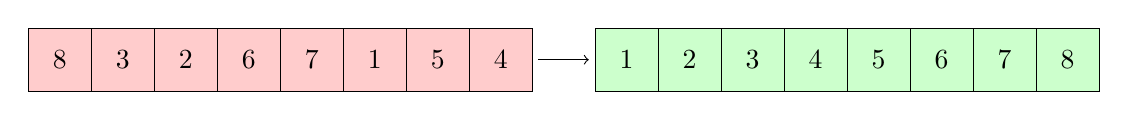
\begin{tikzpicture}[scale=0.8]
            \foreach \x [count=\i] in {8,3,2,6,7,1,5,4} 
            \draw [fill=red!20,shift={(\i,0)}] (0,0) rectangle (1,1) node [midway] {\x};
            \foreach \x [count=\i] in {7,3,2,6,8,1,5,4} 
            \draw [fill=green!20,shift={(\i,0)}] (9,0) rectangle (10,1) node [midway] {\i};
            \draw [->] (9.1,0.5) -- (9.9,0.5);
        \end{tikzpicture}

        按照字典顺序排序字符串
        
        \medskip
        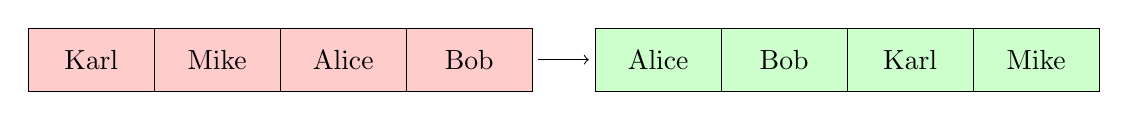
\begin{tikzpicture}[scale=0.8]
            \foreach \x [count=\i] in {Karl,Mike,Alice,Bob} 
            \draw [fill=red!20,shift={({2*\i},0)}] (0,0) rectangle (2,1) node [midway] {\x};
            \foreach \x [count=\i] in {Alice,Bob,Karl,Mike} 
            \draw [fill=green!20,shift={({2*\i},0)}] (9,0) rectangle (11,1) node [midway] {\x};
            \draw [->] (10.1,0.5) -- (10.9,0.5);
        \end{tikzpicture}
    \end{center}
    
\end{frame}


\begin{frame}
    \frametitle{选择排序}
    选择排序的工作原理：通过一轮循环找到最小值，把它放到第一个位置，然后在剩余的数据中再找到最小值，放到第二个位置，以此类推，直到所有值排序完成。
    \begin{enumerate}
      \item 初始状态下，所有元素未排序，即未排序（索引）区间为 $[0, n-1]$ 。
      \item 选取区间 $[0, n-1]$ 中的最小元素，将其与索引 0 处元素交换。完成后，数组前 1 个元素已排序。
      \item 选取区间 $[1, n-1]$ 中的最小元素，将其与索引 1 处元素交换。完成后，数组前 2 个元素已排序。
      \item 以此类推。经过$n-1$轮选择与交换后，数组前$n-1$个元素已排序。
      \item 仅剩的一个元素必定是最大元素，无须排序，因此数组排序完成。
    \end{enumerate}
\end{frame}


\begin{frame}
    \frametitle{图解}
    \begin{center}
        \begin{tikzpicture}[scale=0.8]
            \foreach \x [count=\i] in {8,3,2,6,7,1,5,4} 
            \draw [fill=red!20,shift={(\i,0)}] (0,0) rectangle (1,1) node [midway] {\x};

            \foreach \x [count=\i] in {1,8,3,2,6,7,5,4} 
            \draw [fill=red!20,shift={(\i,-2)}] (0,0) rectangle (1,1) node [midway] {\x};
            \foreach \x [count=\i] in {1} 
            \draw [fill=green!20,shift={(\i,-2)}] (0,0) rectangle (1,1) node [midway] {\x};

            \foreach \x [count=\i] in {1,2,8,3,6,7,5,4} 
            \draw [fill=red!20,shift={(\i,{-4})}] (0,0) rectangle (1,1) node [midway] {\x};
            \foreach \x [count=\i] in {1,2} 
            \draw [fill=green!20,shift={(\i,{-4})}] (0,0) rectangle (1,1) node [midway] {\x};

            
            \foreach \x [count=\i] in {1,2,3,8,6,7,5,4} 
            \draw [fill=red!20,shift={(\i,{-6})}] (0,0) rectangle (1,1) node [midway] {\x};
            \foreach \x [count=\i] in {1,2,3} 
            \draw [fill=green!20,shift={(\i,{-6})}] (0,0) rectangle (1,1) node [midway] {\x};
            
            \foreach \x [count=\i] in {1,2,3,4,8,6,7,5} 
            \draw [fill=red!20,shift={(\i,0)}] (9,0) rectangle (10,1) node [midway] {\x};
            \foreach \x [count=\i] in {1,2,3,4} 
            \draw [fill=green!20,shift={(\i,0)}] (9,0) rectangle (10,1) node [midway] {\x};
            
            \foreach \x [count=\i] in {1,2,3,4,5,8,6,7} 
            \draw [fill=red!20,shift={(\i,{-2})}] (9,0) rectangle (10,1) node [midway] {\x};
            \foreach \x [count=\i] in {1,2,3,4,5} 
            \draw [fill=green!20,shift={(\i,{-2})}] (9,0) rectangle (10,1) node [midway] {\x};
            
            \foreach \x [count=\i] in {1,2,3,4,5,6,8,7} 
            \draw [fill=red!20,shift={(\i,{-4})}] (9,0) rectangle (10,1) node [midway] {\x};
            \foreach \x [count=\i] in {1,2,3,4,5,6} 
            \draw [fill=green!20,shift={(\i,{-4})}] (9,0) rectangle (10,1) node [midway] {\x};

            \foreach \x [count=\i] in {1,2,3,4,5,6,7,8} 
            \draw [fill=red!20,shift={(\i,{-6})}] (9,0) rectangle (10,1) node [midway] {\x};
            \foreach \x [count=\i] in {1,2,3,4,5,6,7} 
            \draw [fill=green!20,shift={(\i,{-6})}] (9,0) rectangle (10,1) node [midway] {\x};

            \draw [->,SteelBlue3] (5,-0.1) -- (5,-0.9) node [midway, right] {第1轮排序};
            \draw [->,shift={(0,-2)},SteelBlue3] (5,-0.1) -- (5,-0.9) node [midway, right] {第2轮排序};
            \draw [->,shift={(0,-4)},SteelBlue3] (5,-0.1) -- (5,-0.9) node [midway, right] {第3轮排序};
            \draw [->,SteelBlue3] (14,1.9) -- (14,1.1) node [midway, right] {第4轮排序};
            \draw [->,shift={(0,-2)},SteelBlue3] (14,1.9) -- (14,1.1) node [midway, right] {第5轮排序};
            \draw [->,shift={(0,-4)},SteelBlue3] (14,1.9) -- (14,1.1) node [midway, right] {第6轮排序};
            \draw [->,shift={(0,-6)},SteelBlue3] (14,1.9) -- (14,1.1) node [midway, right] {第7轮排序};
        \end{tikzpicture}
    \end{center}
    
\end{frame}


\begin{frame}[fragile]
    \frametitle{代码}
    \begin{codeblock}{选择排序}
def selection_sort(nums: list[int]):
    """ 选择排序"""
    n = len(nums)
    # 外循环：未排序区间为 [i, n-1]
    for i in range(n - 1):
        # 内循环：找到未排序区间内的最小元素
        k = i
        for j in range(i + 1, n):
            if nums[j] < nums[k]:
                k = j
                # 记录最小元素的索引
                # 将该最小元素与未排序区间的首个元素交换
        nums[i], nums[k] = nums[k], nums[i]
    \end{codeblock}
\end{frame}


\begin{frame}
    \frametitle{算法时间复杂度}
    \begin{itemize}
      \item 比较次数：$(n-1)+(n-2)+\cdots + 1 = \frac{n(n-1)}{2}$
      \item 交换次数：$n-1$
      \item 总次数：$\frac{(n+2)(n-1)}{2}$
    \end{itemize}
    时间复杂度：$O(n^2)$
\end{frame}


\subsection{冒泡排序}


\begin{frame}
    \frametitle{冒泡排序}
    冒泡排序把一组数据从左边开始进行两两比较，小的放前面，大的放后面，反复比较直到没有数据需要交换为止。
    \begin{enumerate}
      \item 从队首开始，两两比较数值，把大的往后交换，一直到队尾，此时数组的最大元素交换至正确位置；
      \item 从队首开始，对剩余$n-1$个元素执行“冒泡”，将第二大元素交换至正确位置；
      \item 以此类推，经过$n-1$轮“冒泡”后，前$n-1$大的元素都被交换至正确位置。
      \item 仅剩的一个元素必定是最小元素，无须排序，因此数组排序完成。
    \end{enumerate}
\end{frame}


\begin{frame}
    \frametitle{图解\link{https://www.bilibili.com/video/BV1N341127PL}}
    \begin{center}
        \begin{tikzpicture}[scale=0.8]
            \foreach \x [count=\i] in {8,3,2,6,7,1,5,4} 
            \draw [fill=red!20,shift={(\i,0)}] (0,0) rectangle (1,1) node [midway] {\x};

            \foreach \x [count=\i] in {3,2,6,7,1,5,4,8} 
            \draw [fill=red!20,shift={(\i,-2)}] (0,0) rectangle (1,1) node [midway] {\x};
            \foreach \x [count=\i] in {8} 
            \draw [fill=green!20,shift={({9-\i},-2)}] (0,0) rectangle (1,1) node [midway] {\x};

            \foreach \x [count=\i] in {2,3,6,1,5,4,7,8} 
            \draw [fill=red!20,shift={(\i,-4)}] (0,0) rectangle (1,1) node [midway] {\x};
            \foreach \x [count=\i] in {8,7} 
            \draw [fill=green!20,shift={({9-\i},-4)}] (0,0) rectangle (1,1) node [midway] {\x};

            
            \foreach \x [count=\i] in {2,3,1,5,4,6,7,8} 
            \draw [fill=red!20,shift={(\i,{-6})}] (0,0) rectangle (1,1) node [midway] {\x};
            \foreach \x [count=\i] in {8,7,6} 
            \draw [fill=green!20,shift={({9-\i},{-6})}] (0,0) rectangle (1,1) node [midway] {\x};
            
            \foreach \x [count=\i] in {2,1,3,4,5,6,7,8} 
            \draw [fill=red!20,shift={(\i,0)}] (9,0) rectangle (10,1) node [midway] {\x};
            \foreach \x [count=\i] in {8,7,6,5} 
            \draw [fill=green!20,shift={({9-\i},0)}] (9,0) rectangle (10,1) node [midway] {\x};
            
            \foreach \x [count=\i] in {1,2,3,4,5,6,7,8} 
            \draw [fill=red!20,shift={(\i,{-2})}] (9,0) rectangle (10,1) node [midway] {\x};
            \foreach \x [count=\i] in {8,7,6,5,4} 
            \draw [fill=green!20,shift={({9-\i},{-2})}] (9,0) rectangle (10,1) node [midway] {\x};
            
            \foreach \x [count=\i] in {1,2,3,4,5,6,7,8} 
            \draw [fill=red!20,shift={(\i,{-4})}] (9,0) rectangle (10,1) node [midway] {\x};
            \foreach \x [count=\i] in {8,7,6,5,4,3} 
            \draw [fill=green!20,shift={({9-\i},{-4})}] (9,0) rectangle (10,1) node [midway] {\x};

            \foreach \x [count=\i] in {1,2,3,4,5,6,7,8} 
            \draw [fill=red!20,shift={(\i,{-6})}] (9,0) rectangle (10,1) node [midway] {\x};
            \foreach \x [count=\i] in {8,7,6,5,4,3,2} 
            \draw [fill=green!20,shift={({9-\i},{-6})}] (9,0) rectangle (10,1) node [midway] {\x};

            \draw [->,SteelBlue3] (5,-0.1) -- (5,-0.9) node [midway, right] {第1轮冒泡};
            \draw [->,shift={(0,-2)},SteelBlue3] (5,-0.1) -- (5,-0.9) node [midway, right] {第2轮冒泡};
            \draw [->,shift={(0,-4)},SteelBlue3] (5,-0.1) -- (5,-0.9) node [midway, right] {第3轮冒泡};
            \draw [->,SteelBlue3] (14,1.9) -- (14,1.1) node [midway, right] {第4轮冒泡};
            \draw [->,shift={(0,-2)},SteelBlue3] (14,1.9) -- (14,1.1) node [midway, right] {第5轮冒泡};
            \draw [->,shift={(0,-4)},SteelBlue3] (14,1.9) -- (14,1.1) node [midway, right] {第6轮冒泡};
            \draw [->,shift={(0,-6)},SteelBlue3] (14,1.9) -- (14,1.1) node [midway, right] {第7轮冒泡};
        \end{tikzpicture}
    \end{center}
\end{frame}


\begin{frame}[fragile]
    \frametitle{代码}
    \begin{codeblock}{冒泡排序}
def bubble_sort(nums: list[int]):
    """ 冒泡排序"""
    n = len(nums)
    # 外循环：未排序区间为 [0, i]
    for i in range(n - 1, 0, -1):
        # 内循环：将未排序区间 [0, i] 中的最大元素交换至该区间的最右端
        for j in range(i):
            if nums[j] > nums[j + 1]:
                # 交换 nums[j] 与 nums[j + 1]
                nums[j], nums[j + 1] = nums[j + 1], nums[j]
    \end{codeblock}
\end{frame}


\begin{frame}[fragile]
    \frametitle{冒泡排序效率优化}
    如果某轮“冒泡”中没有执行任何交换操作，说明数组已经完成排序，可直接返回结果。因此，可以增加一个标志位 flag 来监测这种情况，一旦出现就立即返回。
    \begin{codeblock}{}
def bubble_sort(nums: list[int]):
    """ 冒泡排序"""
    n = len(nums)
    for i in range(n - 1, 0, -1):
        flag = False  # 初始化标志位
        for j in range(i):
            if nums[j] > nums[j + 1]:
                # 交换 nums[j] 与 nums[j + 1]
                nums[j], nums[j + 1] = nums[j + 1], nums[j]    
                flag = True # 记录交换元素
        if not flag:
            break # 此轮冒泡未交换任何元素，直接跳出
    \end{codeblock}
\end{frame}


\begin{frame}
    \frametitle{算法时间复杂度}
    \begin{itemize}
        \item 冒泡次数：$(n-1)+(n-2)+\cdots + 1 = \frac{n(n-1)}{2}$
      \end{itemize}
      冒泡排序的最差和平均时间复杂度仍为：$O(n^2)$
      \begin{blankblock}{}
        拿数组[1,2,3,4,5,6]为例，这个比较极端完全是有序的，只需要1次冒泡就完成了。在完全有序的情况下，最好的时间复杂度是O(n)。
      \end{blankblock}
\end{frame}


\subsection{插入排序}


\begin{frame}
    \frametitle{插入排序}
    插入排序的工作原理与手动整理一副牌的过程非常相似。具体来说，我们在未排序区间选择一个基准元素，将该元素与其左侧已排序区间的元素逐一比较大小，并将该元素插入到正确的位置。
    \begin{enumerate}
      \item 初始状态下，数组的第 1 个元素已完成排序。
      \item 选取数组的第 2 个元素作为 base ，将其插入到正确位置后，数组的前 2 个元素已排序。
      \item 选取第 3 个元素作为 base ，将其插入到正确位置后，数组的前 3 个元素已排序。
      \item 以此类推，在最后一轮中，选取最后一个元素作为 base ，将其插入到正确位置后，所有元素均已排序。
    \end{enumerate}
\end{frame}


\begin{frame}
    \frametitle{单次插入操作}
    \begin{figure}[htpb]
        \centering
        
\includegraphics[width=\linewidth]{单次插入}
    \end{figure}
\end{frame}


\begin{frame}
    \frametitle{图解}
    \begin{center}
        \begin{tikzpicture}[scale=0.8]
            \foreach \x [count=\i] in {8,3,2,6,7,1,5,4} 
            \draw [fill=red!20,shift={(\i,0)}] (0,0) rectangle (1,1) node [midway] {\x};
            \foreach \x [count=\i] in {8} 
            \draw [fill=green!20,shift={(\i,0)}] (0,0) rectangle (1,1) node [midway] {\x};

            \foreach \x [count=\i] in {3,8,2,6,7,1,5,4} 
            \draw [fill=red!20,shift={(\i,-2)}] (0,0) rectangle (1,1) node [midway] {\x};
            \foreach \x [count=\i] in {3,8} 
            \draw [fill=green!20,shift={(\i,-2)}] (0,0) rectangle (1,1) node [midway] {\x};

            \foreach \x [count=\i] in {2,3,8,6,7,1,5,4} 
            \draw [fill=red!20,shift={(\i,{-4})}] (0,0) rectangle (1,1) node [midway] {\x};
            \foreach \x [count=\i] in {2,3,8} 
            \draw [fill=green!20,shift={(\i,{-4})}] (0,0) rectangle (1,1) node [midway] {\x};

            
            \foreach \x [count=\i] in {2,3,6,8,7,1,5,4} 
            \draw [fill=red!20,shift={(\i,{-6})}] (0,0) rectangle (1,1) node [midway] {\x};
            \foreach \x [count=\i] in {2,3,6,8} 
            \draw [fill=green!20,shift={(\i,{-6})}] (0,0) rectangle (1,1) node [midway] {\x};
            
            \foreach \x [count=\i] in {2,3,6,7,8,1,5,4} 
            \draw [fill=red!20,shift={(\i,0)}] (9,0) rectangle (10,1) node [midway] {\x};
            \foreach \x [count=\i] in {2,3,6,7,8} 
            \draw [fill=green!20,shift={(\i,0)}] (9,0) rectangle (10,1) node [midway] {\x};
            
            \foreach \x [count=\i] in {1,2,3,6,7,8,5,4} 
            \draw [fill=red!20,shift={(\i,{-2})}] (9,0) rectangle (10,1) node [midway] {\x};
            \foreach \x [count=\i] in {1,2,3,6,7,8} 
            \draw [fill=green!20,shift={(\i,{-2})}] (9,0) rectangle (10,1) node [midway] {\x};
            
            \foreach \x [count=\i] in {1,2,3,5,6,7,8,4} 
            \draw [fill=red!20,shift={(\i,{-4})}] (9,0) rectangle (10,1) node [midway] {\x};
            \foreach \x [count=\i] in {1,2,3,5,6,7,8} 
            \draw [fill=green!20,shift={(\i,{-4})}] (9,0) rectangle (10,1) node [midway] {\x};

            \foreach \x [count=\i] in {1,2,3,4,5,6,7,8} 
            \draw [fill=red!20,shift={(\i,{-6})}] (9,0) rectangle (10,1) node [midway] {\x};
            \foreach \x [count=\i] in {1,2,3,4,5,6,7,8} 
            \draw [fill=green!20,shift={(\i,{-6})}] (9,0) rectangle (10,1) node [midway] {\x};

            \draw [->,SteelBlue3] (5,-0.1) -- (5,-0.9) node [midway, right] {第1轮插入};
            \draw [->,shift={(0,-2)},SteelBlue3] (5,-0.1) -- (5,-0.9) node [midway, right] {第2轮插入};
            \draw [->,shift={(0,-4)},SteelBlue3] (5,-0.1) -- (5,-0.9) node [midway, right] {第3轮插入};
            \draw [->,SteelBlue3] (14,1.9) -- (14,1.1) node [midway, right] {第4轮插入};
            \draw [->,shift={(0,-2)},SteelBlue3] (14,1.9) -- (14,1.1) node [midway, right] {第5轮插入};
            \draw [->,shift={(0,-4)},SteelBlue3] (14,1.9) -- (14,1.1) node [midway, right] {第6轮插入};
            \draw [->,shift={(0,-6)},SteelBlue3] (14,1.9) -- (14,1.1) node [midway, right] {第7轮插入};
        \end{tikzpicture}
    \end{center}
\end{frame}


\begin{frame}[fragile]
    \frametitle{代码}
    \begin{codeblock}{插入排序}
def insertion_sort(nums: list[int]):
    """ 插入排序"""
    # 外循环：已排序区间为 [0, i-1]
    for i in range(1, len(nums)):
        base = nums[i]
        j = i - 1
        # 内循环：将 base 插入到已排序区间 [0, i-1] 中的正确位置
        while j >= 0 and nums[j] > base:
            nums[j + 1] = nums[j] # 将 nums[j] 向右移动一位
            j -= 1
        nums[j + 1] = base # 将 base 赋值到正确位置
    \end{codeblock}
\end{frame}


\begin{frame}
    \frametitle{算法时间复杂度}
    \begin{itemize}
        \item 最差情况下，每次插入操作分别需要循环 $n-1$、$n-2$、…、2、1次，求和得到 $\frac{n(n-1)}{2}$ ，因此时间复杂度为 $O(n^2)$
        \item 在遇到有序数据时，插入操作会提前终止。当输入数组完全有序时，插入排序达到最佳时间复杂度$O(n)$
        \item 如果排序记录是随机的，根据概率相同的原则，平均比较和移动的次数约为$n^2/4$次，比冒泡排序和简单选择排序算法性能好一些。
      \end{itemize}
      \begin{blankblock}{}
        虽然冒泡排序、选择排序和插入排序的时间复杂度都为 $O(n^2)$，但在实际情况中，插入排序的使用频率显著高于冒泡排序和选择排序。
      \end{blankblock}
\end{frame}


\subsection{快速排序}


\begin{frame}
    \frametitle{快速排序}
    快速排序是一种基于分治策略的排序算法，运行高效，应用广泛。

    快速排序的核心思想是：选择数组中的某个元素作为“基准数”（哨兵元素），通过一轮排序将要排序的数据分割成独立的两部分，所有小于基准数的元素移到其左侧，而大于基准数的元素移到其右侧。这个基准数可以任取一个，一般取开始、结束或中间位置的一个元素。
    \begin{enumerate}
      \item 选取列表第一个数值作为基准数P，把比P小的数放前面，把比P大的数放后面。
      \item 分别对前面部分和后面部分的数据按照(1)的原则进行排列。
      \item 一直到每一部分只剩一个元素，完成快速排序。
    \end{enumerate}
\end{frame}


\begin{frame}
    \frametitle{按基准数排序}
    \begin{minipage}{0.49\linewidth}
        \begin{center}
            \begin{tikzpicture}[scale=0.9]
                \foreach \x [count=\i] in {2,4,1,0,3,5} 
                \draw [fill=red!20,shift={(\i,0)}] (0,0) rectangle (1,1) node [midway] {\x};
                \draw [fill=green!20,shift={(1,0)}] (0,0) rectangle (1,1) node [midway] {2};
                \draw [->] (1.5,1.2) node [above] {基准值} --  (1.5,1) ;
    
                \foreach \x [count=\i] in {2,4,1,0,3,5} 
                \draw [fill=red!20,shift={(\i,-2)}] (0,0) rectangle (1,1) node [midway] {\x};
                \draw [fill=green!20,shift={(-0.5,-2)}] (0,0) rectangle (1,1) node [midway] {2};
                \draw [->,shift={(-1.5,-2)}] (1.5,1.2) node [above] {基准值} --  (1.5,1) ;
                \draw [fill=green!20,shift={(4,-2)}] (0,0) rectangle (1,1) node [midway] {0};
                \draw [fill=white!20,shift={(1,-2)}] (0,0) rectangle (1,1) node [midway] {2};
                \draw [->,shift={(0,-2)}] (7,1.25)  --   (5,1.25) node [left] {j=3};
                \draw [->,shift={(0,-2)}] (4.2,1.1) .. controls (3,1.5)..(1.5,1.1);
    
                \foreach \x [count=\i] in {0,4,1,0,3,5} 
                \draw [fill=red!20,shift={(\i,-4)}] (0,0) rectangle (1,1) node [midway] {\x};
                \draw [fill=green!20,shift={(-0.5,-4)}] (0,0) rectangle (1,1) node [midway] {2};
                \draw [->,shift={(-1.5,-4)}] (1.5,1.2) node [above] {基准值} --  (1.5,1) ;
                \draw [fill=green!20,shift={(2,-4)}] (0,0) rectangle (1,1) node [midway] {4};
                \draw [fill=white!20,shift={(4,-4)}] (0,0) rectangle (1,1) node [midway] {0};
                \draw [->,shift={(0,-4)}] (1,1.25)  --   (2,1.25) node [right] {i=1};
                \draw [->,shift={(0,-4)}] (2.8,1.1) .. controls (3.5,1.5)..(4.5,1.1);
            \end{tikzpicture}
        \end{center}
    \end{minipage}\hfill
    \begin{minipage}{0.49\linewidth}
        \begin{center}
            \begin{tikzpicture}[scale=0.9]
                \foreach \x [count=\i] in {0,4,1,4,3,5} 
                \draw [fill=red!20,shift={(\i,0)}] (0,0) rectangle (1,1) node [midway] {\x};
                \draw [fill=green!20,shift={(-0.5,0)}] (0,0) rectangle (1,1) node [midway] {2};
                \draw [->,shift={(-1.5,0)}] (1.5,1.2) node [above] {基准值} --  (1.5,1) ;
                \draw [fill=green!20,shift={(3,0)}] (0,0) rectangle (1,1) node [midway] {1};
                \draw [fill=white!20,shift={(2,0)}] (0,0) rectangle (1,1) node [midway] {4};
                \draw [->,shift={(0,0)}] (7,1.25)  --   (4,1.25) node [left] {j=2};
                \draw [->,shift={(0,0)}] (3.2,1.1) .. controls (3,1.5)..(2.5,1.1);

                \foreach \x [count=\i] in {0,1,1,4,3,5} 
                \draw [fill=red!20,shift={(\i,-2)}] (0,0) rectangle (1,1) node [midway] {\x};
                \draw [fill=green!20,shift={(-0.5,-2)}] (0,0) rectangle (1,1) node [midway] {2};
                \draw [->,shift={(-1.5,-2)}] (1.5,1.2) node [above] {基准值} --  (1.5,1) ;
                \draw [fill=white!20,shift={(3,-2)}] (0,0) rectangle (1,1) node [midway] {1};
                \node at (3.5,-0.8) {j=2};
                \node at (3.5,-0.45) {i=2};
                \node at (5,-0.6) {停止查找};
                \draw [->,shift={(0,-2)}] (1,1.25)  --   (3,1.25);
                \draw [->,shift={(2,-2)}] (-2,0) .. controls (0,-0.5)..(1.5,0);

                \foreach \x [count=\i] in {0,1,2,4,3,5} 
                \draw [fill=red!20,shift={(\i,-4)}] (0,0) rectangle (1,1) node [midway] {\x};
                \draw [fill=green!20,shift={(3,-4)}] (0,0) rectangle (1,1) node [midway] {2};
                \draw [->,shift={(2,-4)}] (1.5,1.2) node [above] {基准值} --  (1.5,1) ;
            \end{tikzpicture}
        \end{center}
    \end{minipage}
    
\end{frame}


\begin{frame}
    \frametitle{图解}
    \begin{center}
        \begin{tikzpicture}[scale=0.8]
            \foreach \x [count=\i] in {8,3,2,6,7,1,5,4} 
            \draw [fill=red!20,shift={(\i,0)}] (0,0) rectangle (1,1) node [midway] {\x};

            \foreach \x [count=\i] in {4,3,2,6,7,1,5,8} 
            \draw [fill=red!20,shift={(\i,-2)}] (0,0) rectangle (1,1) node [midway] {\x};
            \draw [fill=green!20,shift={(8,-2)}] (0,0) rectangle (1,1) node [midway] {8};

            \foreach \x [count=\i] in {1,3,2,4,7,6,5,8} 
            \draw [fill=red!20,shift={(\i,{-4})}] (0,0) rectangle (1,1) node [midway] {\x};
            \foreach \x in {4,8} 
            \draw [fill=green!20,shift={(\x,-4)}] (0,0) rectangle (1,1) node [midway] {\x};

            
            \foreach \x [count=\i] in {1,3,2,4,5,6,7,8} 
            \draw [fill=red!20,shift={(\i,{-6})}] (0,0) rectangle (1,1) node [midway] {\x};
            \foreach \x in {1,4,7,8} 
            \draw [fill=green!20,shift={(\x,-6)}] (0,0) rectangle (1,1) node [midway] {\x};
            
            \foreach \x [count=\i] in {1,2,3,4,5,6,7,8} 
            \draw [fill=red!20,shift={(\i,{-8})}] (0,0) rectangle (1,1) node [midway] {\x};
            \foreach \x in {1,2,3,4,5,6,7,8} 
            \draw [fill=green!20,shift={(\x,-8)}] (0,0) rectangle (1,1) node [midway] {\x};

            \draw [->,SteelBlue3] (5,-0.1) -- (5,-0.9) node [midway, right] {第1轮快排};
            \draw [->,shift={(0,-2)},SteelBlue3] (5,-0.1) -- (5,-0.9) node [midway, right] {第2轮快排};
            \draw [->,shift={(0,-4)},SteelBlue3] (5,-0.1) -- (5,-0.9) node [midway, right] {第3轮快排};
            \draw [->,shift={(0,-6)},SteelBlue3] (5,-0.1) -- (5,-0.9) node [midway, right] {第4轮快排};
        \end{tikzpicture}
        \vspace{-1pt}
    \end{center}
\end{frame}






\begin{frame}[fragile]
    \frametitle{代码}
    \begin{codeblock}[firstline=1, lastline =14]{快速排序(1)}
def quick_sort(alist, start, end):
    if start >= end:  # 递归的退出条件
        return
    mid = alist[start]  # 设定起始的基准元素
    low = start  # low为序列左边在开始位置的由左向右移动的游标
    high = end  # high为序列右边末尾位置的由右向左移动的游标
    while low < high:
        # 如果low与high未重合，high(右边)指向的元素大于等于基准元素，则high向左移动
        while low < high and alist[high] >= mid:
            high -= 1
        alist[low] = alist[high]  
        while low < high and alist[low] < mid:
            low += 1
        alist[high] = alist[low] 
    # 退出循环后，low与high重合，此时所指位置为基准元素的正确位置,左边的元素都比基准元素小,右边的元素都比基准元素大
    alist[low] = mid  # 将基准元素放到该位置,
    # 对基准元素左边的子序列进行快速排序
    quick_sort(alist, start, low - 1)  # start :0  low -1 原基准元素靠左边一位
    # 对基准元素右边的子序列进行快速排序
    quick_sort(alist, low + 1, end)  # low+1 : 原基准元素靠右一位  end: 最后

    
    if __name__ == '__main__':
        alist = [54, 26, 93, 17, 77, 31, 44, 55, 20]
        quick_sort(alist, 0, len(alist) - 1)
        print(alist)
    \end{codeblock}
    \vspace{-2pt}
\end{frame}


\begin{frame}[fragile]
    \frametitle{代码}
    \begin{codeblock}[firstline=15, lastline =30, firstnumber=15]{快速排序(2)}
def quick_sort(alist, start, end):
    if start >= end:  # 递归的退出条件
        return
    mid = alist[start]  # 设定起始的基准元素
    low = start  # low为序列左边在开始位置的由左向右移动的游标
    high = end  # high为序列右边末尾位置的由右向左移动的游标
    while low < high:
        # 如果low与high未重合，high(右边)指向的元素大于等于基准元素，则high向左移动
        while low < high and alist[high] >= mid:
            high -= 1
        alist[low] = alist[high]  
        while low < high and alist[low] < mid:
            low += 1
        alist[high] = alist[low] 
    # 退出循环后，low与high重合，此时所指位置为基准元素的正确位置,左边的元素都比基准元素小,右边的元素都比基准元素大
    alist[low] = mid  # 将基准元素放到该位置,
    # 对基准元素左边的子序列进行快速排序
    quick_sort(alist, start, low - 1)  # start :0  low -1 原基准元素靠左边一位
    # 对基准元素右边的子序列进行快速排序
    quick_sort(alist, low + 1, end)  # low+1 : 原基准元素靠右一位  end: 最后

    
if __name__ == '__main__':
    alist = [54, 26, 93, 17, 77, 31, 44, 55, 20]
    quick_sort(alist, 0, len(alist) - 1)
    print(alist)
    \end{codeblock}
\end{frame}


\begin{frame}
    \frametitle{算法时间复杂度}
    \begin{itemize}
      \item 在平均情况下，递归层数为 $\log n$ ，每层中的总循环数为$n$，总体使用 $O(n\log n)$ 时间。
      \item 在最差情况下，每轮操作都将长度为$n$的数组划分为长度为 0 和$n-1$的两个子数组，此时递归层数达到$n$层，每层中的循环数为$n$，总体使用$O(n^2)$时间。
      \item 出现最差情况的概率很低，在绝大多数情况下，快速排序能在$O(n\log n)$的时间复杂度下运行。
    \end{itemize}
\end{frame}


\begin{frame}
    \frametitle{基准数优化}
    快速排序在某些输入下的时间效率可能降低。举一个极端例子，假设输入数组是完全倒序的，由于我们选择最左端元素作为基准数，那么在哨兵划分完成后，基准数被交换至数组最右端，导致左子数组长度为$n-1$、右子数组长度为 0 。如此递归下去，每轮哨兵划分后的右子数组长度都为 0 ，分治策略失效，快速排序退化为“冒泡排序”。

    为了尽量避免这种情况发生，我们可以优化基准数的选取策略。我们可以在数组中选取三个候选元素（通常为数组的首、尾、中点元素），并将这三个候选元素的中位数作为基准数。这样一来，基准数“既不太小也不太大”的概率将大幅提升。当然，我们还可以选取更多候选元素，以进一步提高算法的稳健性。采用这种方法后，时间复杂度劣化至$O(n^2)$的概率大大降低。
\end{frame}


\subsection{归并排序}


\begin{frame}
    \frametitle{归并排序}
    归并排序是一种基于分治策略的排序算法，包含“划分”和“合并”阶段。
    \begin{figure}[htpb]
        \centering
        
\includegraphics[width=.6\linewidth]{归并排序}
    \end{figure}
\end{frame}


\begin{frame}
    \frametitle{算法时间复杂度}
    \begin{itemize}
      \item 划分为$\log n$层
      \item 每层合并的总操作数量为$n$
      \item 总体时间复杂度为$O(n\log n)$
    \end{itemize}
\end{frame}


\subsection{奇葩排序}


\begin{frame}
    \frametitle{猴子排序}
    \begin{quote}
        将无限只猴子置于无限台打字机前，等待无限长的时间，那么猴子也能完整地写出一部《哈姆雷特》。

        \rightline{---波莱尔的无限猴子实验 \qquad}
    \end{quote}
    \vspace{-10pt}
\begin{block}{真猴子实验}
    2003年，英国一所大学的师生给动物园的猴子买了一台电脑和一个键盘。在一个月的时间里，猴子除了胡乱敲键盘外，剩下的时间便是在电脑上进行大小便，最终导致电脑无法正常运行，实验宣告失败。
\end{block}

\begin{block}{程序模拟猴子}
    2004年，电脑模拟的猴子在花费了\num{4.21625e28}年后，终于打出了莎士比亚的剧作《维洛那二绅士》的前十九个字母VALENTINE.Cease to。
\end{block}

\end{frame}


\begin{frame}
    \frametitle{猴子排序}
    基于上述理论，便可以得到猴子排序算法。对于要排序的数组，每一次给它进行一个随机的排序，那么总有一次，它能够变成一个有序的数组。
    \begin{itemize}
      \item 如果运气好，可能一次就搞定。一次成功的幸运猴，时间复杂度就是$O(n)$
      \item 如果运气不好，可能一直都不会成功。永不成功猴，时间复杂度就是$O(\infty)$
    \end{itemize}

        \frametitle{}
        \begin{example}
            尝试用猴子排序算法对10个$1\sim 1000$范围内的数据做排序，看看最终要尝试多少次，花费多长时间？
        \end{example}
\end{frame}


\begin{frame}
    \frametitle{睡眠排序}
    \begin{minipage}{0.44\linewidth}
        \begin{figure}[htpb]
            \centering
            
\includegraphics[width=\linewidth]{睡眠排序}
        \end{figure}
    \end{minipage}\hfill
    \begin{minipage}{0.54\linewidth}
        \small 
        \begin{quote}
            这脑回路，简直是程序员界的一股清流啊，9K说的是年薪吧
        \end{quote}

        \begin{quote}
            多高端呀，都用上多线程了
        \end{quote}

        \begin{quote}
            宝才，公司捡到鬼了
        \end{quote} 
            
        \begin{quote}
            我的老天鹅呀！他真的能用，不过我并不想用2147483637秒去排2147483647个数字。。。
        \end{quote}     

        \begin{quote}
            没有什么问题是睡一觉不能解决的，如果有，就多睡一会儿
        \end{quote}    
        
    \end{minipage}
\end{frame}


\begin{frame}
    \frametitle{睡眠排序}
    构造n个线程，它们和这n个数一一对应。初始化后，线程们开始睡眠，等到对应的数那么多个时间单位后各自醒来，然后输出它对应的数。这样最小的数对应的线程最早醒来，这个数最早被输出，数值越大的线程就会越晚醒来，等所有线程都醒来，排序就结束了。
    \begin{itemize}
      \item 睡眠排序的耗时取决于数组中最大的那个数字，数字越大，耗时越久；
      \item 当数组中存在负数时，运行就会报错，因为线程的睡眠时间不能为负数。
      \item 实际上，睡眠排序面临许多问题
        \begin{itemize}
          \item 输入数据很相近时会有误差
          \item 输入数据很多时，这些线程不能看作是同时启动
          \item 输入数据太大时，运行时间太长
        \end{itemize}
    \end{itemize}
\end{frame}